\documentclass{article}
\usepackage[hidelinks]{hyperref}
%\usepackage{helvetica} % uses helvetica postscript font (download helvetica.sty)
%\usepackage{newcent}   % uses new century schoolbook postscript font 
%\setlength{\textwidth}{5.5in} % set width of text portion
\usepackage{graphicx}
\usepackage{polski}
\usepackage{bm}
\usepackage{amsfonts}
\usepackage{amsmath}
%\usepackage[polish, english]{babel}
%\usepackage[T1]{fontenc} % T1, OT4
\usepackage[utf8]{inputenc}
\usepackage{indentfirst}
\usepackage{float}
\usepackage{enumitem}

\title{Projekt aplikacji do ekstremalnego uczenia maszynowego do klasyfikacji big data}
\author{Abdelkarim Ahmed, Hernik Aleksandra}
\date{}
\begin{document}

\clearpage
\vspace*{\fill}
\begin{center}
\begin{minipage}{.9\textwidth}
\maketitle
\end{minipage}
\end{center}
\vfill % equivalent to \vspace{\fill}
\clearpage

\tableofcontents
\clearpage

\section*{Wprowadzenie}
\addcontentsline{toc}{section}{Wprowadzenie}
Celem pracy jest przetestowanie ELM na wybranych zestawach small data, a następnie big data, przy użyciu służących do tego, istniejących już bibliotek do Pythona i Matlaba.

Ahmed Abdelkarim zajmował się porównywaniem wyników dla big data i~small data przy użyciu Pythona.
Aleksandra Hernik sprawdzała dokładność i~wydajność uczenia dla big data za pomocą Matlaba.

\clearpage
\section*{Wykaz ważniejszych oznaczeń i akronimów}
\addcontentsline{toc}{section}{Wykaz ważniejszych oznaczeń i akronimów}
\begin{itemize}[label={},leftmargin=*]
\item Bias -- wyraz wolny, czyli dodatkowy neuron w warstwie wejściowej niewynikający z danych wejściowych, generujący zawsze +1, ale posiadający wagę
\item Big Data -- dane z liczbą próbek tak dużą, że nie występuje efekt przeuczenia
\item BP -- \textbf{B}ack-\textbf{p}ropagation - propagacja wsteczna
\item ELM -- \textbf{E}xtreme \textbf{L}earning \textbf{M}achine - ekstremalne uczenie maszynowe
\item MLP -- \textbf{M}ulti\textbf{l}ayer \textbf{P}erceptron - perceptron wielowarstwowy
\item SLFN -- \textbf{S}ingle-\textbf{L}ayer \textbf{F}eed-forward \textbf{N}etwork - jednowarstwowa jednokierunkowa sieć neuronowa
\item Small Data -- dane, dla których jest za mało próbek, aby sieć poznała dokładnie model bez przeuczenia
\item SVM -- \textbf{S}upport \textbf{V}ector \textbf{M}achine - maszyna wektorów nośnych
\item Toolbox -- zbiór funkcji stworzonych we wspólnym celu; biblioteka
\end{itemize}
\clearpage
\section{Opracowanie modelu pracy sieci do ekstremalnego uczenia maszynowego ELM}
\subsection{Rys historyczny}
Sieci neuronowe znajdują coraz to nowe zastosowania i stają się jednym z najważniejszych kierunków rozwoju informatyki. Jednak ograniczeniem tej metody jest długotrwały proces uczenia.

W 2004 roku w pracy \textit{Extreme Learning Machine: A New Learning Scheme of Feedforward Neural Networks} Guang-Bin Huang, Qin-Yu Zhu i Chee-Kheong Siew zaproponowali koncepcję ELM, mającą być rozwiązaniem tego problemu. Publikacja ta dotyczyła zastosowania ELM w SLFN. Przedstawiała podstawy teoretyczne do zastosowania tej metody, a także dowodziła zalet tego rozwiązania. Pierwszą jest wspomniana prędkość uczenia. Ponadto w przeciwieństwie do tradycyjnych opartych na gradientach metod, ELM dąży do minimalizacji norm wag, a nie tylko błędu, dzięki czemu osiąga lepszą generalizację. Kolejną istotną własnością ELM jest dopuszczanie zastosowania nieróżniczkowalnych funkcji aktywacji (co nie jest możliwe w tradycyjnych metodach). ELM unika również problemów z minimami lokalnymi i przeuczeniem. 

W tym samym roku Guang-Bin Huang i Chee-Kheong Siew zaproponowali również w artykule \textit{Extreme Learning Machine: RBF Network Case} wariant ELM dla sieci radialnych, których nie dotyczy ta praca. 

Kolejną istotnym wkładem tych autorów do tematu ELM jest opublikowany w 2005 artykuł \textit{Extreme Learning Machine: Theory and Applications}. Prezentowane są w nim wyniki ELM dla testowych danych, które pokazują, że metoda ta pozwala na dobrą klasyfikację, a może działać nawet kilka tysięcy razy szybciej niż tradycyjne metody.

Z wyżej wymienionymi pracami związane są kontrowersje dotyczące rzeczywistej innowacyjności rozwiązania Huanga i innych, a także oskarżenia dotyczące plagiatowania i nieuwzględniania w bibliografii rzeczywistych głównych źródeł pracy -- według nich artykuł dotyczący SLFN opiera się głównie na pracy \textit{Feed Forward Neural Networks With Random Weights} Woutera Schmidta, Martina Kraaijvelda i Roberta Duina z 1992, a artykuł dotyczący sieci radialnych wzoruje się na \textit{Multivariable Functional Interpolation and Adaptive Networks} Davida Broomheada i Davida Lowe'a. Huang wskazał pewne różnice między tymi pracami.

W 2015 roku metoda została również ostro skrytykowana przez Yanna LeCuna, jednego z czołowych specjalistów od sieci neuronowych. Zarzucał pomysłowi prostotę, wskazywał na jego podobieństwo do wcześniejszych pomysłów i wątpił w skuteczność dla większych zestawów danych. Nie odniósł się jednak do wyników zaprezentowanych przez autorów, które pokazują, że rozwiązanie mimo swojej prostoty działa bardzo dobrze.

Teorię o niedostosowaniu ELM do zastosowań big data podważa wydana kilka miesięcy później praca \textit{High-Performance Extreme Learning Machines: A Complete Toolbox for Big Data Applications} autorstwa Antona Akusoka, Kaj-Mikaela Bj\"orka, Yoaba Miche i Amaury'ego Lendasse. Prezentuje ona obiecujące wyniki zastosowania ELM na big data -- dla testowanych danych błąd jest porównywalny, podczas gdy czas uczenia jest mniejszy (od kilku razy dla niektórych metod, nawet do kilku tysięcy razy dla innych). Praca opisuje również udostępniony przez autorów toolbox, implementujący ELM.
\subsection{Założenia dla sieci neuronowych klasy ELM}
Rozważane tu ELM zaliczają się do kategorii SLFN -- poza warstwą wejściową i wyjściową posiadają tylko jedną warstwę ukrytą. Od innych SLFN odróżnia je to, że ELM opierają się na losowym generowaniu neuronów warstwy ukrytej bez późniejszego ich dostosowywania do danych -- dzięki temu, że wszystkie ich parametry, takie jak np. wagi wejściowe, mogą zostać dobrane losowo, są one niezależne od danych trenujących, a w przeciwieństwie do metody BP, wagi wyjściowe są niezależne od wag wejściowych, co pozwala na nieiteracyjne ich wyznaczenie. Takie rozwiązanie zapewnia o kilka rzędów wielkości szybszy czas działania od innych metod, takich jak BP, MLP i SVM. 
%dodać cytowanie Akusoka
\begin{figure}[H]
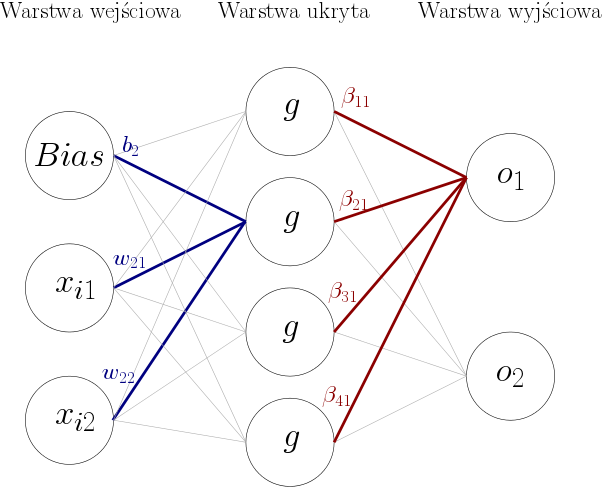
\includegraphics[width=\textwidth]{schemat_sieci.png}
\caption{Schemat SLFN typu ELM}
\end{figure}

Niech $N$ to liczba próbek danych trenujących postaci $(\bm{x}_i, \bm{t}_i) \in \mathbb{R}^n \times \mathbb{R}^m$, gdzie $\bm{x}_i = [x_{i1}, x_{i2}, \dots,  x_{in}]^T$ to dane wejściowe, a $\bm{t}_i = [t_{i1}, t_{i2}, \dots,  t_{im}]^T$ to oczekiwane wyniki. Wtedy dla SLFN z $\bar{N}$ ukrytymi neuronami wyjście dla i-tej próbki danych $(i=1,\dots,N)$ można zapisać jako:
$$\sum_{j=1}^{\bar{N}} \bm{\beta}_j g (\bm{w}_j \cdot \bm{x}_i + b_j)  = \bm{o}_i$$
gdzie $\bm{w}_j = [w_{j1}, w_{j2},\dots,w_{jn}]^T$ to wektor wag łączących warstwę wejściową z j-tym neuronem warstwy ukrytej, $\bm{\beta}_j = [\beta_{j1}, \beta_{j2}, \dots, \beta_{jm}]$ to wektor wag łączących j-ty neuron warstwy ukrytej z warstwą wyjściową, a $b_j$ to bias. W przypadku przybliżenia z zerowym błędem otrzymujemy układ $N$ równań $(i=1,\dots,N)$:
$$\sum_{j=1}^{\bar{N}} \bm{\beta}_j g (\bm{w}_j \cdot \bm{x}_i + b_j)  = \bm{t}_i$$
który można zapisać w postaci macierzowej $\bm{H}\bm{\beta}=\bm{T}$, gdzie: \\
$
H = \begin{bmatrix}
 g(\bm{w}_1 \cdot \bm{x}_1 + b_1) & \cdots & g(\bm{w}_{\bar{N}} \cdot \bm{x}_1 + b_{\bar{N}}) \\
 \vdots & \ddots & \vdots \\
 g(\bm{w}_1 \cdot \bm{x}_N + b_1) & \cdots & g(\bm{w}_{\bar{N}} \cdot \bm{x}_N + b_{\bar{N}})
\end{bmatrix}_{N \times \bar{N}}$, \\
$\bm{\beta} = \begin{bmatrix} \bm{\beta}_1^T \\ \vdots \\ \bm{\beta}_{\bar{N}}^T \end{bmatrix}_{\bar{N} \times m}$ i 
 $ \bm{T} = \begin{bmatrix} \bm{t}_1^T \\ \vdots \\ \bm{t}_N^T \end{bmatrix}_{N \times m}. $\\
i-ta kolumna macierzy $\bm{H}$ (macierzy wyjścia warstwy ukrytej) to wyjście i-tego neuronu warstwy ukrytej dla $\bm{x}_1, \dots, \bm{x}_N$. Jeśli rozważymy macierz $\bm{W}$ jako macierz odpowiednich wag, $\bm{X}$ jako macierz danych wejściowych i $\bm{b}$ jako wektor wyrazów wolnych, otrzymujemy $\bm{H} = g(\bm{XW} + \bm{b})$. W przypadku różnych funkcji aktywacji macierz $\bm{H}$ jest otrzymywana przez konkatenację analogicznie uzyskanych podmacierzy: 
$$\bm{H} = [\bm{H}_1 | \bm{H}_2] = [g_1(\bm{XW}_1 + \bm{b}_1) | g_2(\bm{XW}_2 + \bm{b}_2)].$$ 

Sposób rozwiązania równania $\bm{H}\bm{\beta}=\bm{T}$ jest zależny od liczby próbek $N$ i liczby neuronów warstwy ukrytej $\bar{N}$. W przypadku, gdy $N \leq \bar{N}$, należy zastosować regularyzację w celu otrzymania satysfakcjonującej wydajności. W najczęstszym przypadku $N \gg \bar{N}$ jednak należy zastosować pseudoinwersję Moore'a-Penrose'a:
$$\bm{H}\bm{\beta}=\bm{T} \implies \bm{\beta}=\bm{H}^{\dagger}\bm{T},$$
gdzie 
$$\bm{H}^{\dagger} = (\bm{H}^T \bm{H})^{-1}\bm{H}^T. $$
Błąd trenowania jest wyznaczany za pomocą normy euklidesowej.
%dodać cytowanie Huanga

Możliwości uczenia się ELM zależą między innymi od doboru funkcji transformacji -- w szczególności ważne jest, żeby była ona nieliniowa, ponieważ to jedyne miejsce w całym modelu, w którym może być wykorzystane jakiekolwiek nieliniowe przekształcenie. Możliwe jest wykorzystanie różnych funkcji w różnych neuronach. Dla optymalnej jakości uczenia ważne jest również znormalizowanie danych wejściowych -- jeśli charakterystyki danych wejściowych mają różne rzędy wielkości, relatywnie drobne zmiany większej wartości mogą mieć większe znaczenie niż stosunkowo duże zmiany mniejszych wartości. Normalizacja pozwala na zrównanie wagi zmian wszystkich charakterystyk. \par

W przypadku problemu klasyfikacji, który jest rozważany w tej pracy, rozwiązaniem jest kategoria, dla której wartość na węźle wyjściowym była największa. 
\subsection{Wnioski i uwagi}
Ponieważ ELM jest bardzo szybką metodą, naturalne jest zastosowanie jej do big data -- przy czym tutaj big data oznacza dane takie, że liczba próbek jest wystarczająca, żeby wytrenować sieć bez przeuczania jej, a ograniczeniem jest tylko czas. W przypadku small data próbek jest za mało, żeby sieć mogła dokładnie nauczyć się modelu bez przeuczania. Szybkość uczenia w przypadku big data jest dodatkowo ograniczona sprzętowo -- danych jest zbyt dużo, żeby wszystkie zmieścić do pamięci operacyjnej komputera, co spowalnia dostęp do nich.

\clearpage
\section{Wykonanie implementacji ELM w Pythonie i Matlabie}
\subsection{Założenia dotyczące aplikacji}
Projekt polega na przygotowaniu dwóch aplikacji. Pierwsza jest napisana w języku Python. Druga została stworzona w środowisku Matlab. Celem obu jest przetestowanie nowego modelu sieci neuronowych - Extreme Learning Machine. Programy zapewniają możliwość wytrenowania sieci neuronowej przy użyciu różnych danych i dostarczają informacje, dotyczące czasu trwania i jakości treningu. Dzięki temu będzie możliwe określenie, czy metoda ELM może być uważana za dobrą alternatywę dla tradycyjnych architektur sieci neuronowych, a także w jakich obszarach sprawdzi się najlepiej. Szczególny nacisk został położony na zbadanie działania dla Big Data.

Aplikacje udostępniają następujące funkcjonalności:
\begin{itemize}
\item Przygotowanie danych trenujących i testowych w formie plików csv
\item Trenowanie sieci neuronowej o architekturze ELM
\item Klasyfikacja danych testowych przez wytrenowaną sieć
\item Porównywanie wyników klasyfikacji do spodziewanych rezultatów
\item Analiza jakości klasyfikacji i  czasu trwania treningu
\item Interfejs graficzny
\end{itemize}
Poniższy diagram UML przedstawia zbiór przypadków użycia aplikacji z punktu widzenia użytkownika i systemu, a w następnej tabeli znajduje się ich uszczegółowienie.
\begin{figure}[H]
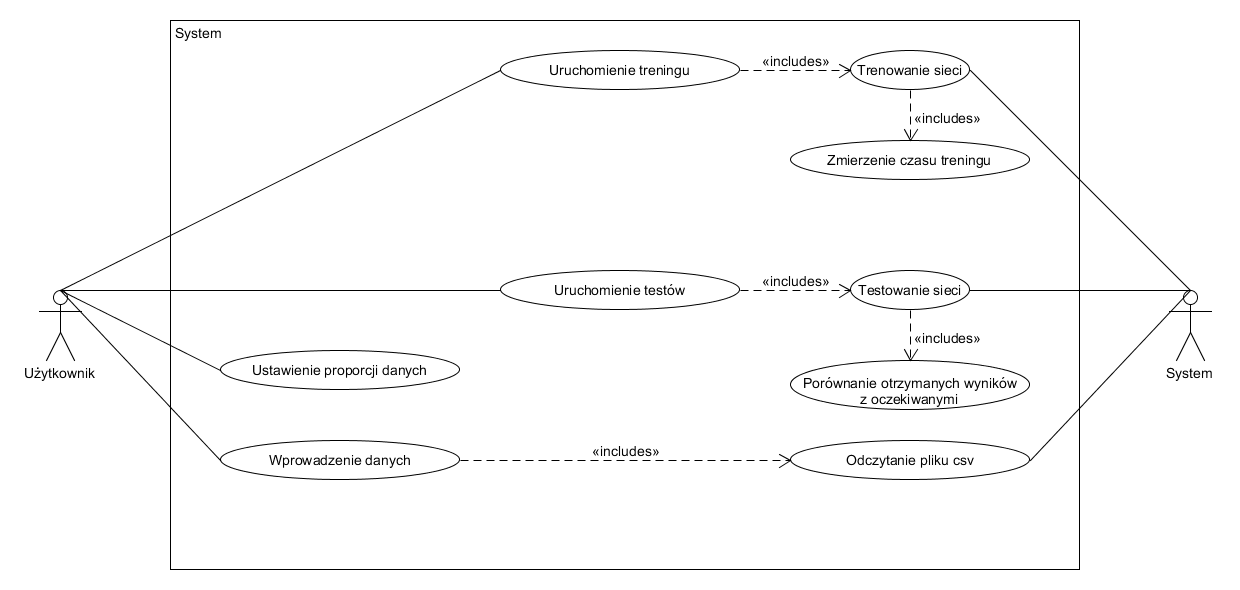
\includegraphics[width=\textwidth]{use_case.png}
\caption{Diagram przypadków użycia}
\end{figure}

\begin{table}[H]
\caption{Opisy przypadków użycia}
\begin{tabular}{|p{3.4cm}|p{5cm}|p{4cm}|}
\hline
\textbf{Nazwa} & \textbf{Opis} & \textbf{Odpowiedź systemu} \\
\hline
Wprowadzenie danych & Wprowadzenie danych używanych do uczenia sieci & Odczytanie pliku csv \\ \hline
Ustawienie proporcji danych & Ustawienie proporcji danych treningowych, testowych i zatwierdzających & Zapisanie wyboru \\ \hline
Uruchomienie treningu & Uruchomienie treningu sieci schematem ELM & Trenowanie sieci i zmierzenie czasu treningu \\ \hline
Uruchomienie testów & Uruchomienie testów sieci wytrenowanej wcześniej schematem ELM & Testowanie sieci i porównanie otrzymanych wyników z oczekiwanymi \\
\hline
\end{tabular}
\end{table}

Wymagania niefunkcjonalne aplikacji zostały określone następująco:
\begin{table}[H]
\caption{Lista wymagań niefunkcjonalnych}
\begin{tabular}{|l|l|p{9.4cm}|}
\hline
\textbf{Obszar} & \textbf{Numer} & \textbf{Opis} \\
\hline
Użyteczność & 1 & Aplikacje muszą działać na komputerach wydziałowych \\
 & 2 & Aplikacje powinny mieć przejrzysty interfejs graficzny \\
 & 3 & Wykresy wyświetlane w aplikacji powinny być czytelne \\
\hline
Wydajność & 4 & Działanie w oparciu o ELM powinno dawać o kilka rzędów wielkości szybszy czas uczenia niż tradycyjne metody \\
\hline 
Inne & 5 & Wykonanie aplikacji w językach Python i MATLAB \\
& 6 & Dobrze udokumentowany kod \\
\hline
\end{tabular}
\end{table}
\subsection{Projekt aplikacji sieci ELM w Pythonie}
\subsection{Projekt aplikacji sieci ELM w Matlabie}
\subsection{Wnioski i uwagi}
\begin{itemize}
\item Automatyczne testy, sprawdzające główną funkcjonalność programu - trening sieci - nie zostaną utworzone. Istotą projektu jest przeanalizowanie otrzymywanych, a nie otrzymanie z góry zaplanowanych wyników.
\item Nie zostały postawione wymagania związane z niezawodnością i utrzymaniem. Aplikacje służą wyłącznie jako narzędzia do przetestowania nowej technologii, więc jedynym wymaganiem jest działanie w momencie przeprowadzania testów. Ta kwestia może ulec zmianie, jeśli testy wypadną korzystnie dla ELM.
\item Wydajność jest raczej oczekiwaniem, nie wymaganiem. Z prac, na których bazowany jest projekt wynika, że metoda powinna być szybka, jednak założenia projektu polegają na sprawdzeniu, a nie przyjęciu tej tezy. Ponadto nie zostały zaimplementowane inne metody uczenia sieci neuronowych, więc precyzyjna ocena wydajności byłaby trudna.
\end{itemize}
\clearpage
\section{Trening ELM dla wybranych benchmarków big data i small data}
\subsection{Opis wybranych benchmarków}
\subsection{Trening dla instancji klasy small data}
\subsection{Trening dla instancji klasy big data}
\subsection{Wnioski i uwagi}

\clearpage
\section{Eksperymenty obejmujące instancje klasyfikacji wraz z badaniem ich wydajności}
\clearpage
\section*{Podsumowanie}
\addcontentsline{toc}{section}{Podsumowanie}

\clearpage
\section*{Bibliografia}
\addcontentsline{toc}{section}{Bibliografia}
\begin{thebibliography}{9}

\bibitem{akusok}
  A. Akusok, K.-M. Björk, Y. Miche, A. Lendasse,
  \emph{High-Performance Extreme Learning Machines: A Complete Toolbox for Big Data Applications},

\end{thebibliography}
TODO dobre referencje
\begin{itemize}
\item  \textit{}
\item G.-B. Huang, L. Chen, C.-K. Siew, \textit{Extreme learning machine: Theory and applications} 
\item http://elmorigin.wixsite.com/originofelm
\end{itemize}
\clearpage
\addcontentsline{toc}{section}{Spis rysunków}
\listoffigures
\clearpage
\addcontentsline{toc}{section}{Spis tabel}
\listoftables
\clearpage
\section*{Dodatek. Instrukcja obsługi aplikacji}
\addcontentsline{toc}{section}{Dodatek. Instrukcja obsługi aplikacji}

\clearpage
\end{document}













